The user then clicks on the E21\_Person1 in the R2RML mapping and selects Augment Data to discover new data to integrate into artist records.  
Karma then parses R2RML mappings in its repository that describe crm:E21\_Person.
From these mappings, Karma generates a candidate set of linked data sources to integrate, identifies meaningful object and data properties, and presents this to the user as illustrated in Figure~\ref{fig:search-screenshot}.

To aid the user, Karma also estimates how many of the user's artists are likely to have these properties in the linked data source.  
Karma does this by testing the artists' URIs against Bloom filters that it created when generating RDF triples and then associated with the Predicate Object Maps of an R2RML mapping.  
Karma's estimation helps the user avoid an expensive and unfruitful join very cheaply since the Bloom filters trade a small false positive rate for a much smaller data structure than a perfect hash, all while supporting arbitrary set operations.  
\begin{figure*}[t]
\centering
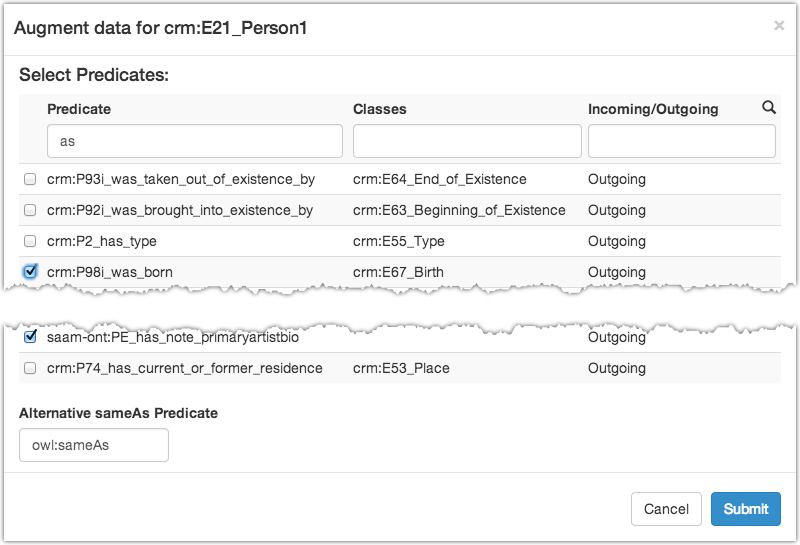
\includegraphics[width=4.9in]{images/5-search.png}
\vspace{-5mm}
\caption{A Karma user selects CIDOC CRM object and data properties discovered from other sources to augment crm:E21\_Person}
\vspace{-21pt}
\label{fig:search-screenshot}
\end{figure*}